\section{Metodologia}\label{sec:metodologia}

Esta seção reúne os modelos físicos que definem o simulador estocástico, a formulação da função de estado limite dependente do tempo, o procedimento de construção do emulador (incluindo a camada temporal de aprendizado de máquina) e a ponte entre a distribuição emulada e as grandezas de gestão de ativos (probabilidade de falha, tempo até a falha, RUL e métricas de risco).

% =====================================================================
% 4.1 CORROSAO INDUZIDA POR CARBONATACAO  (Section_2 do grupo)
% =====================================================================
\subsection{Corros\~ao induzida por carbonata\c{c}\~ao}
\label{subsec:carbonatacao}

\subsubsection{Fenomenologia}
\label{subsub:fenomenologia}

A corrosão desencadeada pela carbonatação difere substancialmente de outros mecanismos agressivos por sua natureza química global, governada pela redução progressiva da alcalinidade da matriz cimentícia. Enquanto agentes como os íons cloreto perfuram a camada passiva de forma localizada (corrosão por \textit{pites}), a carbonatação avança como uma frente ácida que reduz o pH do concreto a níveis inferiores a 9, promovendo a despassivação generalizada de toda a superfície da armadura afetada. Essa perda de proteção em larga escala resulta em corrosão uniforme, caracterizada pela formação volumosa de óxidos expansivos ao longo da barra, o que gera tensões de tração no concreto e culmina em fissuração intensa e destacamento do cobrimento, mesmo antes da perda crítica de seção transversal do aço \parencite{tuutti1982}.

O processo inicia-se com a difusão do dióxido de carbono atmosférico (CO$_2$) através da rede de poros do concreto. O CO$_2$ reage com a umidade dos poros e com os produtos de hidratação do cimento, predominantemente o hidróxido de cálcio (Ca(OH)$_2$), levando à formação de carbonato de cálcio (CaCO$_3$), conforme a Equação~\eqref{eq:carbonation}:

\begin{equation}\label{eq:carbonation}
\mathrm{Ca(OH)_2 + CO_2 \rightarrow CaCO_3 + H_2O}
\end{equation}

Em condições normais, o concreto mantém um ambiente altamente alcalino (pH entre 12,6 e 13,5), que sustenta uma película passiva estável de óxidos sobre a superfície do aço, conferindo proteção efetiva contra a corrosão. O avanço progressivo da frente de carbonatação, contudo, reduz o pH a valores inferiores a 9, despassivando a armadura e tornando o aço suscetível à corrosão generalizada na presença de oxigênio e umidade. O processo de corrosão é tipicamente dividido em duas fases: \textit{iniciação}, durante a qual a armadura permanece passivada enquanto a frente avança em direção a ela, e \textit{propagação}, na qual a película protetora é destruída e a corrosão ativa se desenvolve \parencite{tuutti1982}.

A velocidade e a profundidade da carbonatação são influenciadas por diversos fatores ambientais e de material, tais como: a concentração de CO$_2$ (níveis mais elevados aceleram a reação); a umidade relativa do ar (a carbonatação é mais intensa em faixas intermediárias, tipicamente 50\%--70\%); a qualidade do concreto (relação água/cimento, tipo de cimento e porosidade determinam a facilidade de ingresso do CO$_2$); e a espessura do cobrimento, que atua como barreira física \parencite{possan2010}.

\begin{figure}[htpb!]
    \centering
    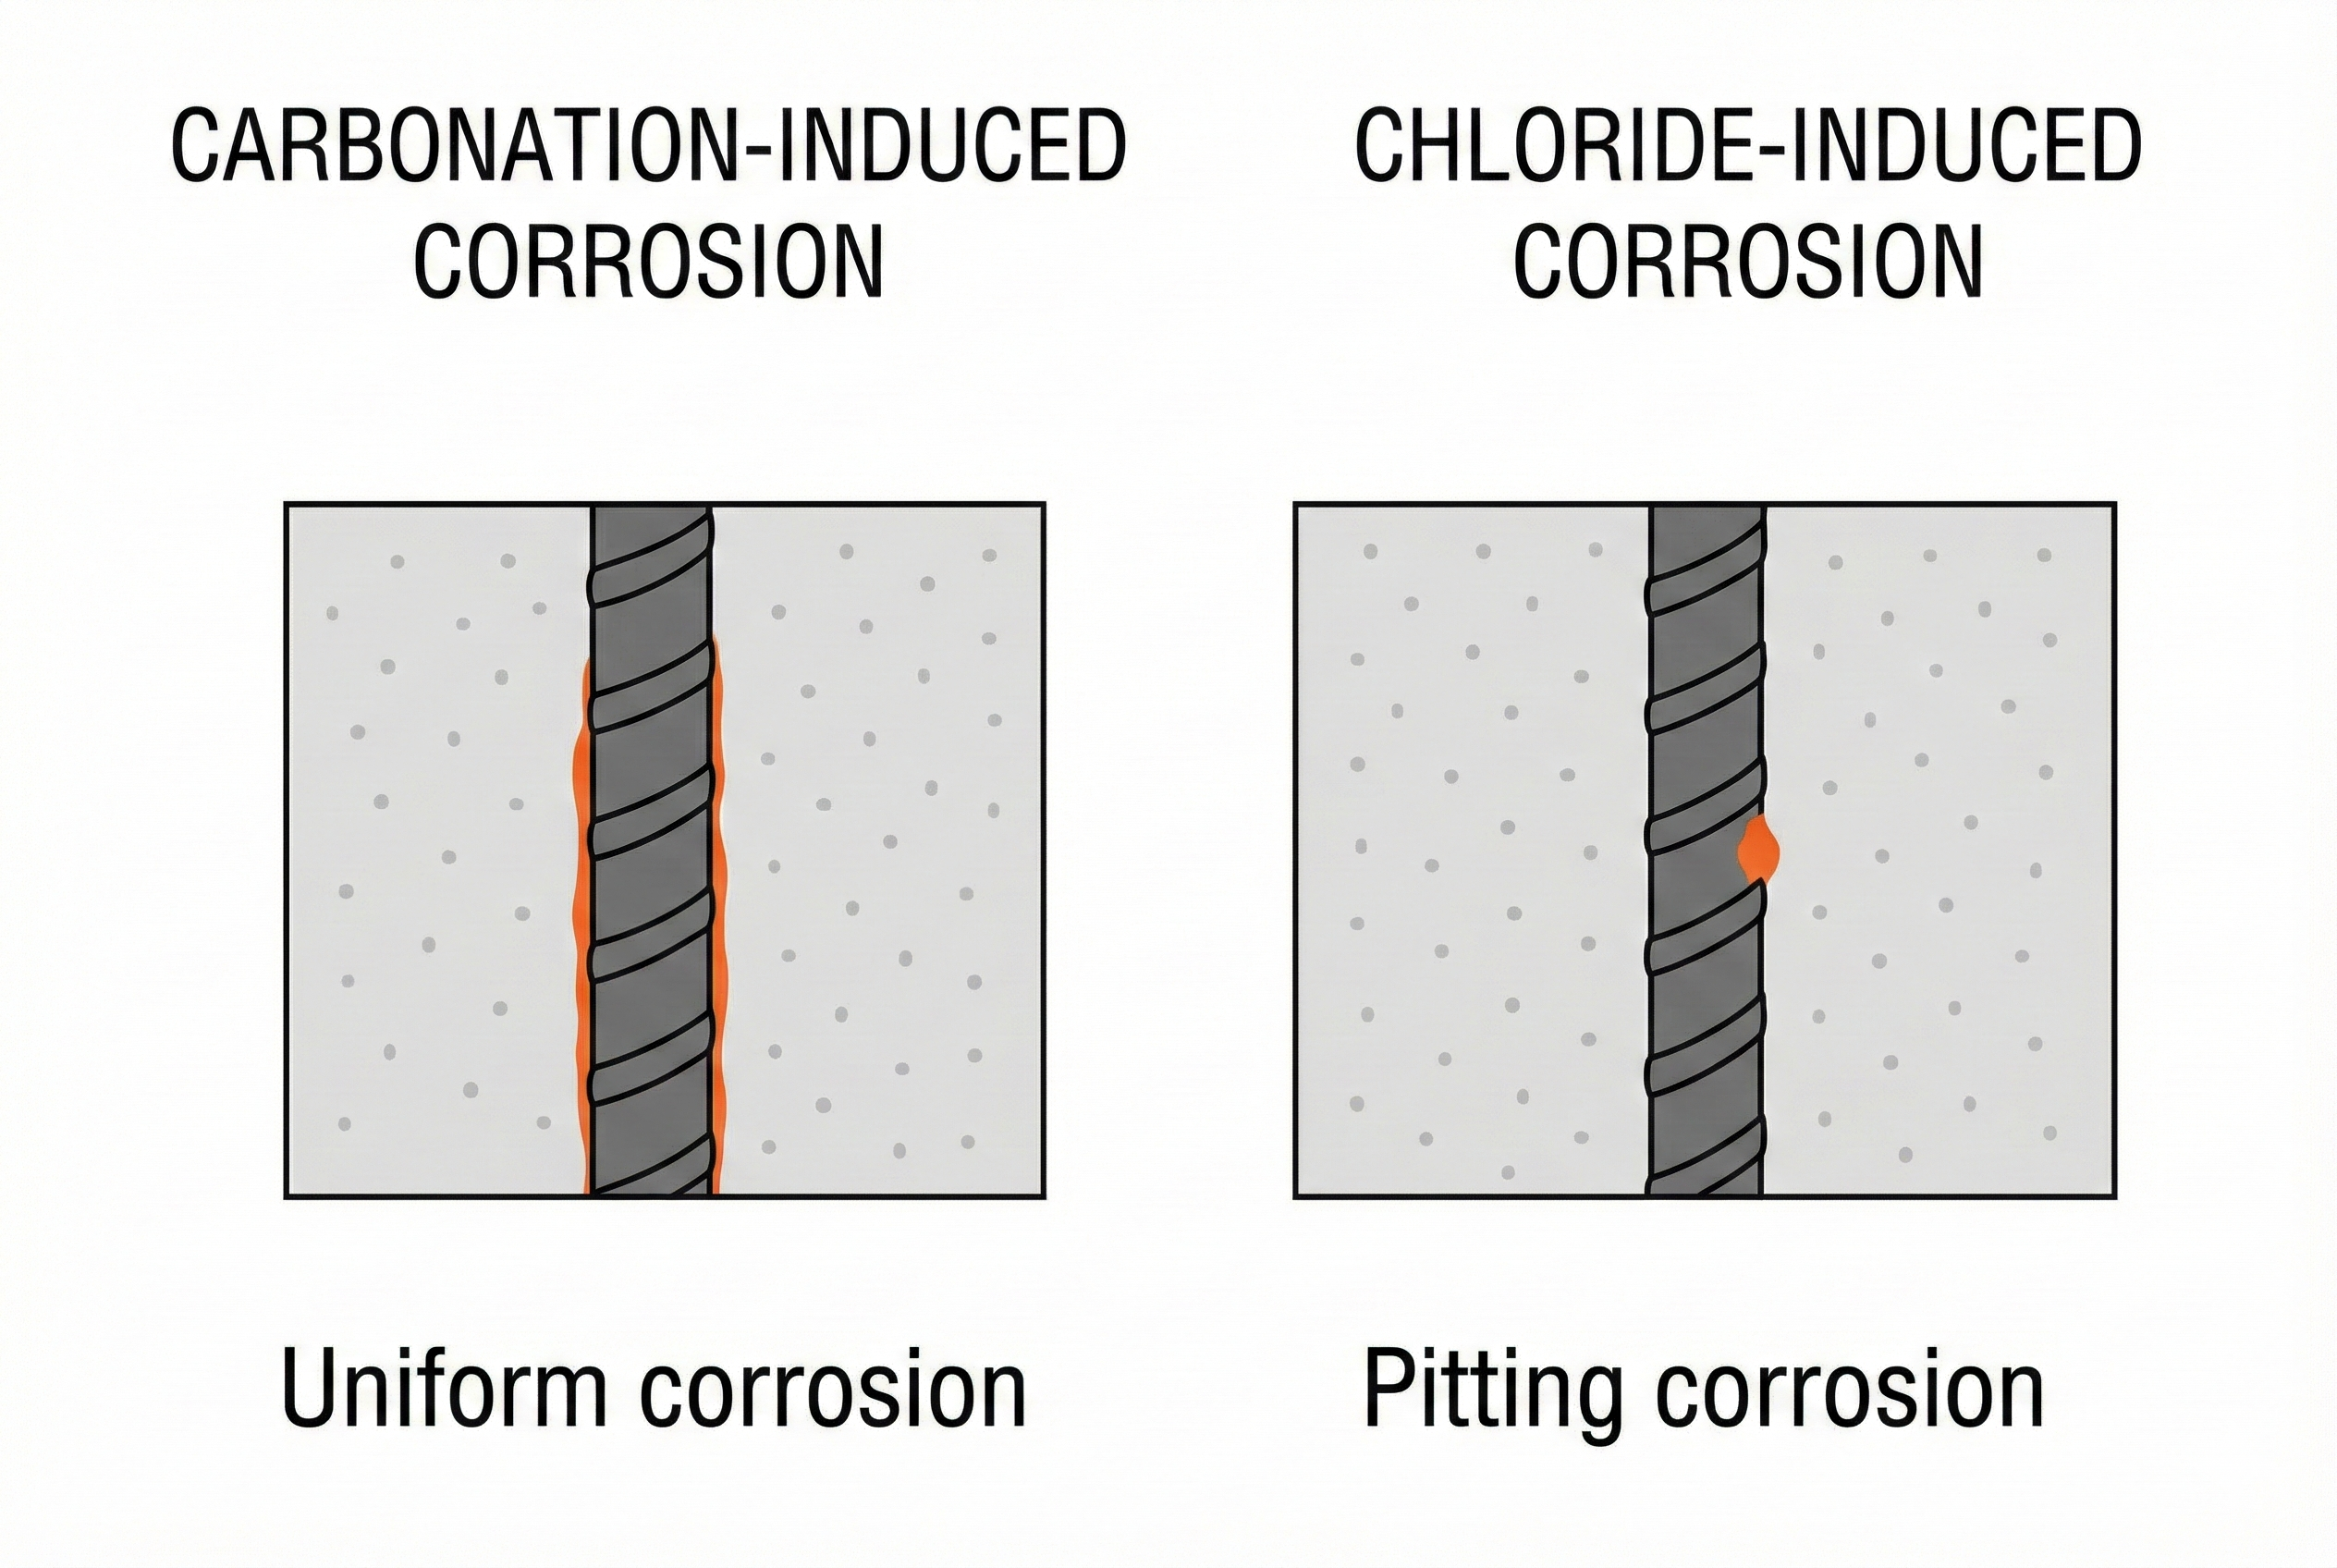
\includegraphics[width=0.5\linewidth]{z_corrosion_en.png}
    \caption{Diferenças entre os mecanismos de corrosão localizada (cloretos) e generalizada (carbonatação). \falta{traduzir a figura para o português; se mantida em inglês, indicar na legenda}}
    \label{fig:z_corrosion_en}
\end{figure}

\subsubsection{Modelo de avan\c{c}o da frente de carbonata\c{c}\~ao}
\label{subsec:modelo_possan}

O modelo proposto por \textcite{possan2010} oferece uma abordagem paramétrica para a previsão da profundidade de carbonatação $y(t)$ em estruturas de concreto armado, integrando variáveis de material e de ambiente. A formulação matemática, expressa na Equação~\eqref{eq:y}, estima o avanço da frente de carbonatação ao longo do tempo, considerando a influência da resistência à compressão ($f_c$), do tipo de cimento, das adições minerais, da concentração de CO$_2$ e da umidade relativa ($UR$):

\begin{equation}\label{eq:y}
y(t) = k_c \cdot \left( \frac{20}{f_c} \right)^{k_{fc}} \cdot \left( \frac{t}{20} \right)^{\frac{1}{2}} \cdot \exp \left[ \frac{k_{ad} \cdot ad^{\frac{3}{2}}}{40 + f_c} + \frac{k_{CO_2} \cdot CO_2^{\frac{1}{2}}}{60 + f_c} - \frac{k_{UR} \cdot (UR - 0{,}58)^2}{100 + f_c} \right] \cdot k_{ce}
\end{equation}

\noindent em que $k_c$, $k_{fc}$, $k_{ad}$, $k_{CO_2}$, $k_{UR}$ e $k_{ce}$ são coeficientes calibrados em função do tipo de cimento e da condição de exposição, $ad$ é o teor de adições e $t$ é o tempo de exposição em anos. Em formulações simplificadas, frequentemente utilizadas em análises de confiabilidade, o avanço da frente reduz-se à clássica lei da raiz do tempo,

\begin{equation}\label{eq:raiz_t}
y_{\mathrm{carb}}(t) = k\,\sqrt{t},
\end{equation}

\noindent na qual o coeficiente de carbonatação $k$ (mm/$\sqrt{\text{ano}}$) condensa o efeito conjunto de material e ambiente, podendo ser obtido por regressão de perfis medidos como $k = y/\sqrt{t}$.

A despassivação ocorre quando a frente de carbonatação atinge o nível da armadura, isto é, quando $y_{\mathrm{carb}}(t) \geq c_{\mathrm{nom}}$, em que $c_{\mathrm{nom}}$ é o cobrimento nominal. O instante de iniciação da corrosão, $t_{\mathrm{ini}}$, é definido como a primeira raiz dessa condição. A partir desse ponto inicia-se a fase de propagação, tratada na Seção~\ref{subsec:resistencia_residual}.

\subsubsection{Base de dados e perfis de refer\^encia}
\label{subsec:dataset}

Para a caracterização probabilística do fenômeno, este estudo apoia-se em uma base de dados abrangente de progressão da carbonatação em estruturas de concreto, composta por 20.000 amostras, obtida em trabalho anterior do grupo \parencite{couto2025}. A base incorpora variáveis numéricas e categóricas que caracterizam as condições ambientais, as propriedades dos materiais e os fatores temporais que influenciam a profundidade de carbonatação: concentração atmosférica de CO$_2$ (\%), resistência à compressão aos 28 dias $f_c$ (MPa), umidade relativa $UR$ (\%), tempo de exposição $t$ (anos), tipo de cimento (seis classes segundo a \textcite{nbr16697}: CP~V-ARI, CP~II-E, CP~II-F, CP~II-Z, CP~III e CP~IV) e condição de exposição (interna protegida, externa protegida e externa desprotegida). A variável-alvo é a profundidade de carbonatação $y$ (mm). A Tabela~\ref{tab:statistics} apresenta as estatísticas descritivas das variáveis numéricas.

\begin{table}[htpb!]
    \centering
    \small
    \caption{Estatísticas descritivas das variáveis numéricas da base de dados de carbonatação ($n = 20.000$) \parencite{couto2025}.}
    \label{tab:statistics}
     \begin{tabular}{lrrrr}
    \toprule
     & \textbf{média} & \textbf{desvio} & \textbf{mín.} & \textbf{máx.} \\
    \midrule
    \textbf{CO$_2$ (\%)} & 0,16 & 0,08 & 0,03 & 0,30 \\
    \textbf{$f_c$ (MPa)} & 34,90 & 8,66 & 20,00 & 50,00 \\
    \textbf{$UR$ (\%)} & 59,94 & 17,31 & 30,00 & 90,00 \\
    \textbf{$t$ (anos)} & 49,93 & 29,32 & 0,00 & 100,00 \\
    \textbf{prof. carbonatação (mm)} & 16,59 & 12,84 & 0,00 & 119,71 \\
    \bottomrule
    \end{tabular}
\end{table}

Em \textcite{couto2025}, sete modelos de aprendizado de máquina foram treinados sobre essa base para a predição da profundidade de carbonatação, com validação cruzada de 10 dobras; os modelos de melhor desempenho (rede neural MLP e \textit{Histogram-based Gradient Boosting}) atingiram $R^2 = 0{,}99$ no conjunto de teste, enquanto regressões lineares limitaram-se a $R^2 \approx 0{,}54$, evidenciando a forte não linearidade do fenômeno. Esses resultados validam a base de dados como fonte de perfis representativos de carbonatação e justificam o uso de metamodelos não lineares no presente arcabouço. \falta{se desejado, recuperar aqui a tabela completa de desempenho dos 7 modelos e as figuras de dispersão previsto vs.\ observado do trabalho anterior (candidato a Ap\^endice)}

A análise dos perfis de profundidade permitiu determinar coeficientes de carbonatação médios por classe de resistência. Para a condição de exposição interna protegida, que apresentou as maiores taxas de carbonatação, obtiveram-se $k_{20} = 5{,}8$, $k_{30} = 3{,}8$, $k_{40} = 2{,}3$ e $k_{50} = 1{,}7$~mm/$\sqrt{\text{ano}}$ para as classes C20 a C50, respectivamente, conforme ilustrado na Figura~\ref{fig:z_carbonation_profile}.

\begin{figure}[htpb!]
        \centering
        
\includegraphics[width= 0.60\textwidth]{z_carbonation_profile.png}
        \caption{Perfis de carbonatação para exposição interna protegida e coeficientes de carbonatação por classe de resistência. \falta{traduzir rótulos da figura para o português}}
        \label{fig:z_carbonation_profile}
\end{figure}

\subsubsection{Perfil temporal de CO$_2$ atmosf\'erico}
\label{subsec:co2}

Para modelar a evolução temporal da concentração atmosférica de CO$_2$ --- parâmetro fundamental das simulações de degradação de longo prazo --- adotou-se uma abordagem baseada em registros históricos e instrumentais. Para o período de 1900 a 1950, os dados derivam de registros paleoclimáticos de alta resolução extraídos de testemunhos de gelo antártico (Law Dome), mantidos pelo NOAA/NCEI \parencite{noaa_law_dome}. A partir de 1950, o modelo ancora-se em medições atmosféricas diretas e contínuas do observatório de Mauna Loa, mantidas pelo NOAA Global Monitoring Laboratory \parencite{noaa_gml}.

Para uso nesta pesquisa, foi ajustada uma regressão analítica por partes que simula esse perfil de acumulação de CO$_2$, com coeficiente de determinação $R^2 = 0{,}99$. O arcabouço matemático divide a série temporal em três regimes contínuos de crescimento antropogênico, ilustrados na Figura~\ref{fig:evolution_co2}: crescimento linear lento entre 1900 e 1950, crescimento linear acelerado entre 1950 e 2000 e crescimento quadrático após 2000, capturando a intensificação contemporânea das emissões globais. \falta{apresentar as equações dos três trechos da regressão por partes}

\begin{figure}[htpb!]
    \centering
    
\includegraphics[width=0.5\linewidth]{z_graph_1900_co2.png}
    \caption{Regressão por partes da concentração atmosférica de CO$_2$ simulada de 1900 a 2150. \falta{traduzir rótulos da figura}}
    \label{fig:evolution_co2}
\end{figure}

Como ilustração da aplicação dos modelos descritos, simulações paramétricas projetaram o avanço da carbonatação para o período estendido de 1900 a 2150. As Figuras~\ref{fig:evolution_fck} e \ref{fig:evolution_h} apresentam a evolução temporal da frente de carbonatação, destacando a influência direta da classe de resistência ($f_{ck}$) e da umidade relativa sobre a taxa de degradação. Para fins de avaliação de vida útil, adotou-se uma linha de referência em 30~mm, correspondente a um cobrimento normativo típico \parencite{nbr6118}, indicando o limiar teórico de despassivação da armadura. Observa-se, em particular, a aceleração da degradação em ambientes de umidade intermediária (65\%) em comparação com ambientes mais secos (50\%) ou mais úmidos (80\%).

\begin{figure}[htpb!]
    \centering
    \begin{subfigure}[b]{0.48\textwidth}
        \centering
        
\includegraphics[width=\linewidth]{z_graph_1900_fck.png}
        \caption{Influência da classe de resistência $f_{ck}$ ($UR = 65\%$).}
        \label{fig:evolution_fck}
    \end{subfigure}
    \hfill
    \begin{subfigure}[b]{0.48\textwidth}
        \centering
        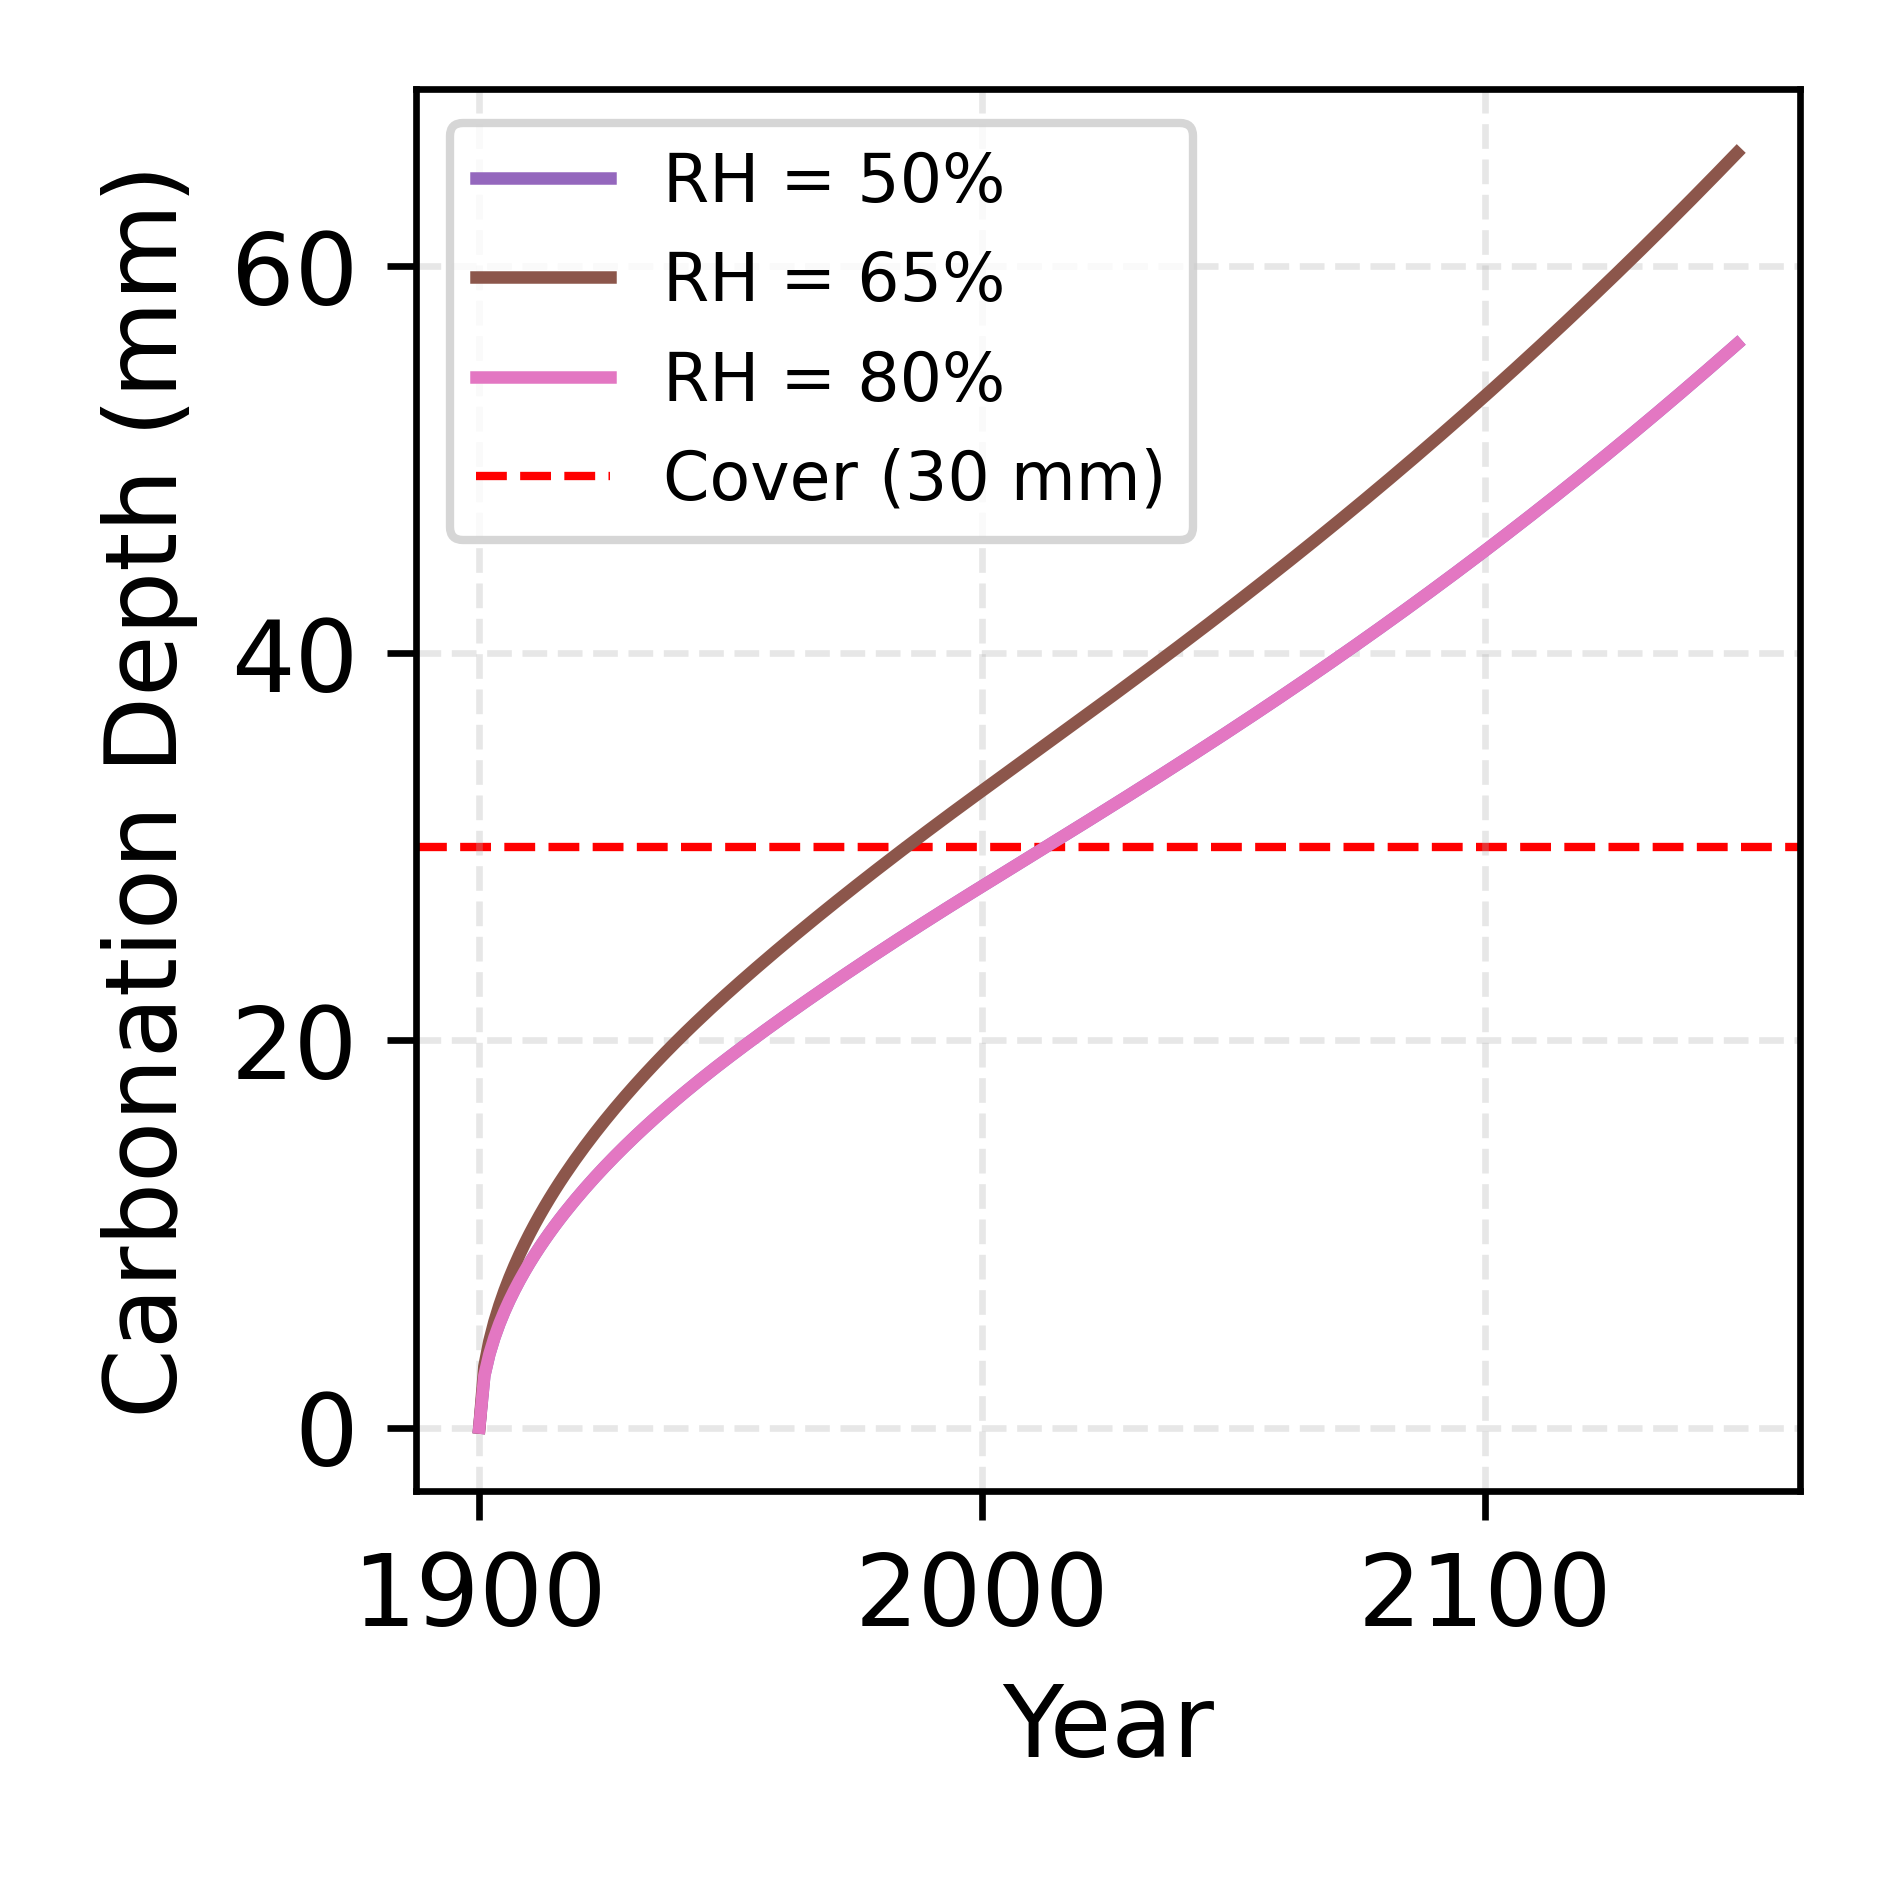
\includegraphics[width=\linewidth]{z_graph_1900_h.png}
        \caption{Influência da umidade relativa ($f_{ck} = 30$~MPa).}
        \label{fig:evolution_h}
    \end{subfigure}
    \caption{Evolução temporal da frente de carbonatação (1900--2150) com linha de referência no cobrimento normativo de 30~mm. \falta{traduzir rótulos das figuras}}
    \label{fig:evolucao_carb}
\end{figure}

% =====================================================================
% 4.2 RESISTENCIA RESIDUAL E FUNCAO DE ESTADO LIMITE  (Section_3)
% =====================================================================
\subsection{Resist\^encia residual \`a flex\~ao e fun\c{c}\~ao de estado limite}
\label{subsec:resistencia_residual}

Apresentam-se aqui os modelos para a previsão da capacidade resistente residual de vigas de concreto armado sujeitas à corrosão induzida por carbonatação. A formulação combina (i) o cálculo normativo da resistência à flexão conforme a \textcite{nbr6118} e (ii) a modelagem físico-química dos efeitos da corrosão sobre a área de aço e sobre a aderência aço--concreto, com base em \textcite{azad2010}, \textcite{val1997} e \textcite{peng2016}. Ao final, define-se a função de estado limite dependente do tempo que constitui a resposta do simulador estocástico a ser emulado.

\subsubsection{Momento resistente da se\c{c}\~ao \'integra}
\label{subsub:mrd0}

O cálculo de vigas de concreto armado sem corrosão ($t \leq t_{\mathrm{ini}}$) segue as diretrizes da \textcite{nbr6118}. O momento fletor resistente de cálculo ($M_{Rd}$) é determinado pelo equilíbrio de forças na seção transversal, considerando o comportamento não linear dos materiais e o diagrama retangular simplificado de tensões no concreto comprimido. As resistências de cálculo do concreto, $f_{cd}$, e do aço, $f_{yd}$, são obtidas pela aplicação dos respectivos coeficientes de ponderação ($\gamma_c$ e $\gamma_s$), e os parâmetros geométricos do bloco de tensões ($\lambda_c$, $\alpha_c$) são definidos em função da resistência característica $f_{ck}$.

Para seções retangulares com armadura simples, o equilíbrio entre a força normal de compressão no concreto e a força de tração na armadura escreve-se como

\begin{equation}\label{eq:equilibrio}
f_\alpha(\beta) = R_c(\beta) - R_s(\beta) = \sigma_{cd}\, \lambda_c\, (\beta d)\, b_w \;-\; \sigma_s(\beta)\, A_s = 0,
\end{equation}

\noindent em que $\beta = x/d$ é a profundidade relativa da linha neutra, $x$ é a profundidade da linha neutra, $b_w$ é a largura da seção, $d$ é a altura útil, $A_s$ é a área de armadura tracionada, $\sigma_{cd}$ é a tensão de cálculo no concreto comprimido e $\sigma_s$ é a tensão na armadura, obtida do diagrama elastoplástico definido pela norma. Devido às não linearidades física e geométrica, a raiz de $f_\alpha(\beta) = 0$ é obtida numericamente pelo método da bisseção em um intervalo predefinido. Convergido o valor de $x$, o momento resistente é calculado pela Equação~\eqref{eq:mrd_lim_resumida}:

\begin{equation}\label{eq:mrd_lim_resumida}
M_{Rd} = \sigma_{cd} \cdot (\lambda_c \cdot x \cdot b_w) \cdot \left(d - \tfrac{1}{2} \lambda_c x\right),
\end{equation}

\noindent em que o termo entre parênteses representa o braço de alavanca interno. Esse valor estabelece a linha de base de desempenho da estrutura antes do início da degradação por corrosão, denotada $M_{Rd,0}$.

\subsubsection{Propaga\c{c}\~ao da corros\~ao e resist\^encia residual}
\label{subsub:residual}

Após o início da corrosão, considerado no instante $t_{\mathrm{ini}}$ definido na Seção~\ref{subsec:modelo_possan}, o modelo incorpora dois efeitos de degradação: (i) a perda de seção transversal das barras e (ii) a redução da aderência aço--concreto.

\paragraph{Taxa de corros\~ao ajustada pela temperatura.}
A taxa de corrosão não é considerada constante. Seguindo \textcite{peng2016}, a taxa é ajustada em função da temperatura ambiente $T(t)$ e da classe de exposição:

\begin{equation}\label{eq:i_cor_t}
i_{\mathrm{corr}}(T) = i_{\mathrm{corr},20} \left[ 1 + K \cdot (T - 20) \right],
\qquad
K =
\begin{cases}
0{,}073, & T > 20\,^\circ\mathrm{C}, \\
0{,}025, & T < 20\,^\circ\mathrm{C}, \\
0, & T = 20\,^\circ\mathrm{C},
\end{cases}
\end{equation}

\noindent em que $i_{\mathrm{corr},20}$ ($\mu$A/cm$^2$) é a taxa de corrosão de referência a 20\,$^\circ$C.

\paragraph{Perda de di\^ametro e \'area efetiva.}
Definindo o período de propagação como $t_{\mathrm{corr}} = t - t_{\mathrm{ini}}$, a redução do diâmetro original $d_{s0}$ (mm) decorre da lei de Faraday e é dada por \parencite{val1997, azad2010}:

\begin{equation}\label{eq:d_cor}
d_{s}(t) = d_{s0} - 0{,}0232 \cdot i_{\mathrm{corr}} \cdot t_{\mathrm{corr}},
\end{equation}

\noindent de modo que a área efetiva da armadura com $n_b$ barras torna-se

\begin{equation}\label{eq:as_t}
A_{s}(t) = n_b\, \frac{\pi\, d_{s}(t)^2}{4}.
\end{equation}

\paragraph{Redu\c{c}\~ao da ader\^encia.}
A perda de aderência entre o aço corroído e o concreto é representada por um coeficiente redutor $C_f$ \parencite{azad2010}:

\begin{equation}\label{eq:c_f}
C_f = \min\!\left[\,1,\; \frac{5{,}0}{\, d_{s0}^{0{,}54} \left( i^{*}_{\mathrm{corr}} \cdot t_{\mathrm{corr}} \cdot 365 \right)^{0{,}19}}\right],
\end{equation}

\noindent em que $i^{*}_{\mathrm{corr}} = i_{\mathrm{corr}}/1000$ é expresso em A/mm$^2$ e $t_{\mathrm{corr}}$ em anos.

\paragraph{Momento resistente degradado.}
A resistência à flexão degradada é então calculada recompondo o equilíbrio seccional da Equação~\eqref{eq:equilibrio} com a área corroída $A_s(t)$ e aplicando o coeficiente de aderência:

\begin{equation}\label{eq:m_res}
M_{Rd,\mathrm{cor}}(t) = C_f \cdot M_{Rd}\!\left(A_{s}(t)\right).
\end{equation}

\subsubsection{Fun\c{c}\~ao de estado limite dependente do tempo}
\label{subsec:funcao_g}

Obtido o momento resistente degradado, avalia-se o estado limite último de flexão pela comparação entre resistência e solicitação. O momento solicitante característico total é

\begin{equation}\label{eq:ms}
M_S = M_{Gk} + M_{Qk},
\end{equation}

\noindent em que $M_{Gk}$ e $M_{Qk}$ são, respectivamente, os momentos característicos das ações permanentes e variáveis. A margem de segurança no instante $t$ --- a função de estado limite do problema --- é definida como

\begin{equation}\label{eq:funcao_g}
g(\mathbf{X}, t) = M_{Rd,\mathrm{cor}}(\mathbf{X}, t) - M_S(\mathbf{X}),
\end{equation}

\noindent em que $\mathbf{X}$ reúne todas as variáveis aleatórias do problema (propriedades de material, geometria, ambiente e ações). A interpretação física é direta:

\begin{equation}\label{eq:dominio_falha}
\begin{cases}
g(\mathbf{X}, t) \geq 0, & \text{estrutura segura (estado limite não violado)}, \\[4pt]
g(\mathbf{X}, t) < 0,  & \text{ocorrência do estado limite último}.
\end{cases}
\end{equation}

O valor de $g$ indica a distância, em termos de momento fletor, entre a capacidade residual da seção corroída e a demanda estrutural. A redução progressiva de $g$ ao longo do tempo reflete a deterioração da armadura longitudinal, tanto pela perda de seção quanto pela redução da aderência. Note-se que, em razão das variáveis latentes do problema (heterogeneidade do material, flutuações ambientais, incerteza de modelo), $g(\mathbf{X}, t)$ é, para cada par $(\mathbf{x}, t)$, uma \textit{variável aleatória}, e não um valor determinístico --- precisamente a estrutura de um simulador estocástico (Seção~\ref{subsec:simulador}). Este procedimento, repetido para todos os instantes da simulação e para todas as amostras estocásticas, permitiria em princípio a determinação de curvas de confiabilidade e da probabilidade de falha por simulação direta de Monte Carlo; o custo proibitivo dessa estratégia para análises de ciclo de vida é justamente o que motiva o emulador proposto.

\falta{a NOTA do grupo sugere um estado limite alternativo de durabilidade $g = c_{\mathrm{nom}} - y_{\mathrm{carb}}(t)$ (despassiva\c{c}\~ao: ``cobrimento menos ataque''), mais simples e diretamente lig\'avel ao Exemplo~2. Ver sugest\~ao no plano de melhorias.}

% =====================================================================
% 4.3 CONSTRUCAO DO EMULADOR DEPENDENTE DO TEMPO  (Section_4 temporal)
% =====================================================================
\subsection{Constru\c{c}\~ao do emulador dependente do tempo}
\label{subsec:construcao_emulador}

Definidos o simulador estocástico (Seção~\ref{subsec:funcao_g}) e o núcleo estatístico do emulador (Seção~\ref{sec:emuladores}), descreve-se aqui o procedimento concreto de construção do emulador PCE--GLD e sua extensão ao domínio temporal.

\subsubsection{Plano de experimentos e ajuste local}
\label{subsub:doe}

O treinamento do emulador PCE--GLD segue os passos:

\begin{enumerate}
    \item \textbf{Plano de experimentos:} um conjunto de $M$ pontos amostrais $\{\mathbf{x}^{(1)}, \dots, \mathbf{x}^{(M)}\}$ é gerado por Amostragem por Hipercubo Latino (LHS) \parencite{mckay1979}.
    \item \textbf{Avaliações estocásticas:} para cada ponto $\mathbf{x}^{(j)}$, o simulador estocástico original é executado $N$ vezes, gerando um conjunto amostral local da resposta, $\mathcal{Y}^{(j)}$.
    \item \textbf{Ajuste local da GLD:} o método dos momentos, implementado no PyGLAM com o otimizador BFGS, é utilizado para estimar os parâmetros locais ótimos $\hat{\boldsymbol{\lambda}}^{(j)}$ para cada $\mathcal{Y}^{(j)}$.
    \item \textbf{Estimação dos coeficientes da PCE:} a partir dos pares $\{\mathbf{x}^{(j)}, \hat{\boldsymbol{\lambda}}^{(j)}\}_{j=1}^M$, os coeficientes $a_{i, \boldsymbol{\alpha}}$ da Equação~\eqref{eq:pce_lambda} são calculados para cada $\lambda_i$.
\end{enumerate}

\subsubsection{Emula\c{c}\~ao dependente do tempo}
\label{subsub:temporal}

O processo de carbonatação é inerentemente dependente do tempo, exigindo que a evolução da distribuição da margem de segurança seja capturada ao longo de toda a vida em serviço da estrutura. Para tanto, o arcabouço PCE--GLD é estendido para incluir o tempo $t$ como variável de entrada contínua. Nesse esquema de emulação temporal, os parâmetros $\boldsymbol{\lambda}$ da GLD são avaliados em passos de tempo discretos, e um metamodelo de aprendizado de máquina (Seção~\ref{sec:ml}) é subsequentemente treinado para mapear o espaço conjunto de variáveis físicas $\mathbf{X}$ e tempo $t$ nos parâmetros da distribuição.

A base de treinamento do emulador temporal é construída avaliando-se o simulador estocástico em $N_t$ passos de tempo discretos $\{t_1, t_2, \dots, t_{N_t}\}$ (e.g., 0, 10, 20, 50 e 80 anos). Para cada passo $t_m$, um conjunto de $M$ amostras do vetor de entrada $\mathbf{X}^{(j)}$ é avaliado, produzindo os parâmetros locais correspondentes $\hat{\boldsymbol{\lambda}}^{(j, m)}$ via PyGLAM. A base de dados resultante $\mathcal{D}$ é definida como:

\begin{equation}
\mathcal{D} = \left\{ \left( \mathbf{x}^{(j)}, t_m \right), \hat{\boldsymbol{\lambda}}^{(j, m)} \right\} \quad \text{para } j=1,\dots,M \text{ e } m=1,\dots,N_t
\label{eq:dataset_temporal}
\end{equation}

Para prever os parâmetros da GLD em um instante arbitrário $t^*$, emprega-se o modelo de ML de múltiplas saídas descrito na Seção~\ref{subsec:redes_neurais}, que aprende o mapeamento não linear $f: (\mathbf{X}, t) \to \mathbb{R}^4$:

\begin{equation}
\hat{\boldsymbol{\lambda}}(\mathbf{X}, t) \approx \mathcal{M}_{ML}(\mathbf{X}, t; \mathbf{w}).
\label{eq:ml_temporal}
\end{equation}

Ao incluir o passo de tempo como entrada explícita, o emulador interpola os valores de $\{\lambda_1, \dots, \lambda_4\}$ entre os anos simulados, fornecendo uma evolução contínua da distribuição da margem de segurança ao longo de todo o período de análise. Duas salvaguardas são adotadas: (i) a restrição de validade $\lambda_2 > 0$ é imposta na saída do regressor (Seção~\ref{subsec:redes_neurais}); e (ii) parâmetros que exibam baixa sensibilidade às entradas podem ser excluídos do treinamento e representados por seu valor médio, decisão tomada caso a caso a partir de análise exploratória (ver Seção~\ref{subsec:exemplo1}).

\subsubsection{M\'etricas de valida\c{c}\~ao do emulador}
\label{subsec:metricas}

A similaridade estatística entre os dados de referência (\textit{ground truth}, obtidos por simulação direta) e as amostras geradas pelo emulador é avaliada por um conjunto complementar de métricas, todas aplicadas em pontos e instantes \textit{não utilizados no treinamento}:

\paragraph{Testes de ader\^encia.} O teste de Kolmogorov--Smirnov (KS) \parencite{massey1951} quantifica a máxima distância entre as funções de distribuição acumuladas empíricas, sendo sensível a discrepâncias globais; o teste de Anderson--Darling (AD) \parencite{anderson1952, scholz1987} pondera fortemente as caudas, sendo adequado para detectar desvios nas regiões extremas, justamente as mais relevantes para confiabilidade.

\paragraph{Compara\c{c}\~ao de quantis.} Erros relativos nos quantis $\{0{,}001;\, 0{,}01;\, 0{,}5;\, 0{,}99;\, 0{,}999\}$ localizam a origem de eventuais discrepâncias e quantificam diretamente a qualidade da aproximação na cauda inferior, região que governa a probabilidade de falha.

\paragraph{Diverg\^encia de Kullback--Leibler.} Para duas densidades $p(x)$ (referência) e $q(x)$ (emulador), a entropia relativa \parencite{kullback1951, cover2006}

\begin{equation}
D(p \,\|\, q) = \int p(x)\, \log \frac{p(x)}{q(x)}\, dx
\label{eq:kl_continua}
\end{equation}

\noindent é não negativa e anula-se se, e somente se, $p = q$. Embora não seja simétrica nem satisfaça a desigualdade triangular, é frequentemente útil interpretá-la como uma medida de ``distância'' entre distribuições, fornecendo um escalar global de qualidade do emulador.

% =====================================================================
% 4.4 DA DISTRIBUICAO EMULADA A RUL  (Section_5)
% =====================================================================
\subsection{Da distribui\c{c}\~ao emulada \`a vida \'util remanescente}
\label{subsec:rul}

Esta subseção estabelece a ponte entre a distribuição condicional de $g(\mathbf{X},t)$ fornecida pelo emulador e as grandezas de interesse para a gestão de ativos: a probabilidade de falha dependente do tempo, a distribuição do tempo até a falha, a vida útil remanescente probabilística e suas métricas de risco, além do modelo de intervenção de manutenção.

\subsubsection{Probabilidade de falha e fun\c{c}\~ao de confiabilidade}
\label{subsec:pf}

Dado que o emulador fornece, para qualquer instante $t$, os parâmetros $\hat{\boldsymbol{\lambda}}(\mathbf{X},t)$ da GLD que aproxima a distribuição de $g$, a probabilidade de falha instantânea é obtida diretamente da função quantílica, sem necessidade de amostragem:

\begin{equation}
p_f(t) = \mathbb{P}\left[\, g(\mathbf{X}, t) \leq 0 \,\right] = F_{g(t)}(0) = Q^{-1}_{t}(0),
\label{eq:pf_t}
\end{equation}

\noindent em que $F_{g(t)}$ é a CDF da margem de segurança no instante $t$ e $Q_t$ a correspondente função quantílica emulada. O índice de confiabilidade generalizado associado é $\beta(t) = -\Phi^{-1}\!\left[p_f(t)\right]$, em que $\Phi$ é a CDF normal padrão \parencite{melchers2018}. A função de confiabilidade da estrutura, entendida como a probabilidade de sobrevivência até $t$, é denotada $R(t)$; para processos de degradação monotônica, como a perda de seção por corrosão, a aproximação $R(t) \approx 1 - p_f(t)$ é adequada, uma vez que trajetórias de $g$ que cruzam o zero não retornam ao domínio seguro. \falta{se forem consideradas ações variáveis com flutuação no tempo (problema de primeira passagem não monotônico), discutir a correção via taxa de ultrapassagem (\textit{outcrossing rate}) ou deixar explícita a hipótese de monotonicidade}

\subsubsection{Tempo at\'e a falha e vida \'util remanescente}
\label{subsec:ttf_rul}

Para cada realização $\mathbf{x}$ das variáveis de entrada, o tempo até a falha é definido como o primeiro instante em que a margem de segurança se anula:

\begin{equation}
T(\mathbf{x}) = \inf\left\{\, t \geq 0 \,:\, g(\mathbf{x}, t) \leq 0 \,\right\}.
\label{eq:ttf}
\end{equation}

A distribuição de $T$ é obtida de forma extremamente eficiente a partir do emulador: amostram-se realizações de $\mathbf{X}$, avalia-se a trajetória contínua $\hat{g}(\mathbf{x}, t)$ por meio da GLD interpolada no tempo e identifica-se a raiz da Equação~\eqref{eq:ttf} para cada amostra. Dado um instante de inspeção $t_{\mathrm{insp}}$, no qual se constata a sobrevivência da estrutura, a vida útil remanescente é a variável aleatória condicionada

\begin{equation}
\mathrm{RUL}(t_{\mathrm{insp}}) = \left(\, T - t_{\mathrm{insp}} \,\middle|\, T > t_{\mathrm{insp}} \right),
\label{eq:rul}
\end{equation}

\noindent cuja distribuição completa --- e não apenas seu valor esperado --- constitui o produto central deste trabalho \parencite{si2011}. Dela extraem-se o valor esperado $\mathbb{E}[\mathrm{RUL}]$, a mediana e quantis inferiores (e.g., $P_5$), estes últimos de particular interesse para decisões conservadoras.

\subsubsection{M\'etricas de risco: VaR e CVaR}
\label{subsec:var_cvar}

Para apoiar a tomada de decisão sob incerteza, métricas de risco baseadas em cauda são derivadas da distribuição de RUL, a saber, o \textit{Value-at-Risk} (VaR) e o \textit{Conditional Value-at-Risk} (CVaR) \parencite{rockafellar2000}. Enquanto a caracterização probabilística completa da RUL fornece a visão abrangente do comportamento do sistema, essas métricas escalares oferecem indicadores conservadores focados em cenários adversos, particularmente relevantes para o planejamento de manutenção.

O VaR ao nível de confiança $\alpha$ representa o quantil inferior da distribuição de RUL,

\begin{equation}
\mathrm{VaR}_\alpha = \inf\left\{\, r \,:\, F_{\mathrm{RUL}}(r) \geq \alpha \,\right\},
\label{eq:var}
\end{equation}

\noindent indicando a vida remanescente mínima esperada com confiança $(1-\alpha)$. O CVaR, por sua vez, corresponde ao valor esperado da RUL condicionado aos valores abaixo do limiar do VaR,

\begin{equation}
\mathrm{CVaR}_\alpha = \mathbb{E}\left[\, \mathrm{RUL} \,\middle|\, \mathrm{RUL} \leq \mathrm{VaR}_\alpha \,\right],
\label{eq:cvar}
\end{equation}

\noindent contabilizando explicitamente o comportamento da cauda e fornecendo uma medida de risco mais conservadora.

\subsubsection{Modelagem de interven\c{c}\~oes de manuten\c{c}\~ao}
\label{subsec:manutencao}

O emulador proposto habilita a avaliação rápida de cenários de manutenção, uma vez que cada cenário exige apenas reavaliações da GLD interpolada, e não novas execuções do simulador original. Considera-se uma intervenção no instante $t_{\mathrm{man}}$ --- por exemplo, a remoção do concreto carbonatado, limpeza das armaduras e recomposição do cobrimento com argamassa de reparo realcalinizante --- cujo efeito sobre a função de estado limite é modelado por dois mecanismos \parencite{frangopol2011, vannoortwijk2009}:

\begin{enumerate}
    \item \textbf{Recuperação da margem de segurança:} o momento resistente é restaurado a uma fração $\rho \in (0, 1]$ de seu valor íntegro, $M_{Rd,\mathrm{cor}}(t_{\mathrm{man}}^{+}) = \rho \cdot M_{Rd,0}$, em que $\rho$ reflete a eficácia do reparo ($\rho = 1$ corresponde à recuperação total; valores típicos \falta{indicar faixa adotada e justificar com referência});
    \item \textbf{Reinício do relógio de iniciação:} a recomposição do cobrimento realcaliniza a vizinhança da armadura, de modo que um novo período de iniciação se desenvolve no material de reparo, $t_{\mathrm{ini}}^{\mathrm{novo}} = t_{\mathrm{man}} + \Delta t_{\mathrm{ini}}$, com $\Delta t_{\mathrm{ini}}$ governado pelo coeficiente de carbonatação do material de reparo $k_{\mathrm{rep}}$ \falta{definir distribuição de $k_{\mathrm{rep}}$; na ausência de dados, adotar $k_{\mathrm{rep}} = k$ como hipótese conservadora}.
\end{enumerate}

A trajetória resultante da margem de segurança assume o típico formato ``dente de serra'' das estruturas mantidas, e a Equação~\eqref{eq:ttf} é avaliada sobre a trajetória composta. A comparação entre as distribuições de RUL com e sem intervenção quantifica o \textit{ganho probabilístico de vida útil} proporcionado pela manutenção:

\begin{equation}
\Delta \mathrm{RUL} = \mathrm{RUL}_{\mathrm{com\;man.}}(t_{\mathrm{insp}}) - \mathrm{RUL}_{\mathrm{sem\;man.}}(t_{\mathrm{insp}}).
\label{eq:delta_rul}
\end{equation}

Adicionalmente, o emulador permite determinar de forma praticamente instantânea o \textit{instante normativo de intervenção}, definido como o primeiro tempo em que a probabilidade de falha atinge um alvo de norma,

\begin{equation}
t_{\mathrm{man}}^{*} = \inf\left\{\, t \,:\, \beta(t) \leq \beta_{\mathrm{alvo}} \,\right\},
\label{eq:t_man_otimo}
\end{equation}

\noindent adotando-se, por exemplo, $\beta_{\mathrm{alvo}} = 1{,}5$ para estados limites de serviço/durabilidade, em consonância com as recomendações do \textcite{fib2006} e do \textcite{jcss2001}. Ressalta-se que este trabalho emprega a política de limiar da Equação~\eqref{eq:t_man_otimo} como demonstração da utilidade do emulador para decisões de manutenção; a otimização completa de custo de ciclo de vida, envolvendo custos de inspeção, reparo e falha, constitui extensão natural e é apontada como trabalho futuro.
